\chapter{Dasar Teori}
\label{chap:Dasar Teori}

\section{jsoup}
\label{sec:jsoup}

\textit{Web scraping} adalah teknik mendapatkan informasi dari sebuah situs web secara otomatis\cite{Vargiu:2013}. Dalam bahasa Java, \textit{web scraping} dapat diimplementasikan menggunakan \textit{library} jsoup\cite{jsoup}. API yang disediakan oleh jsoup dapat digunakan untuk mengekstrak dan memanipulasi data HTML. 

Subbab-subbab berikut menjelaskan beberapa kelas dari jsoup.

\subsection{Jsoup}

Kelas ini merupakan inti untuk mengakses fungsi jsoup. Seluruh \textit{method} dalam kelas ini merupakan \texttt{static} \textit{method} sehingga kelas ini tidak perlu dikonstruksi. Salah satu \textit{method} yang dimiliki kelas ini adalah sebagai berikut:
\begin{itemize}
	\item \textbf{public static Connection connect(String url)} \\
		Berfungsi untuk membuat koneksi baru dengan suatu situs web. \\
		\textbf{Parameter:}
		\begin{itemize}
			\item \textbf{url} URL situs web dengan protokol HTTP atau HTTPS.
		\end{itemize}
		\textbf{Kembalian:} koneksi dengan situs web.
\end{itemize}

\subsection{Connection}

Kelas ini merupakan \texttt{interface} yang menyediakan pengambilan data dari situs web. Beberapa \textit{method} yang dimiliki kelas ini adalah sebagai berikut:

\begin{itemize}
	\item \textbf{Connection cookies(Map<String,String> cookies)} \\
		Berfungsi untuk menambahkan \textit{cookie}. \\
		\textbf{Parameter:}
		\begin{itemize}
			\item \textbf{cookies} \texttt{Map} dari \textit{cookie}.
		\end{itemize}
		\textbf{Kembalian:} koneksi yang sama tetapi sudah diubah.
		
		\item \textbf{Connection data(String key, String value)} \\
		Berfungsi untuk menambahkan parameter data yang bisa dikirim melalui metode HTTP GET atau POST. \\
		\textbf{Parameter:}
		\begin{itemize}
			\item \textbf{key} kunci data.
			\item \textbf{value} nilai data.
		\end{itemize}
		\textbf{Kembalian:} koneksi yang sama tetapi sudah diubah.
		
		\item \textbf{Connection method(Connection.Method method)} \\
		Berfungsi untuk mengatur metode permintaan HTTP, GET atau POST. Metode pengiriman secara \textit{default} adalah GET\\
		\textbf{Parameter:}
		\begin{itemize}
			\item \textbf{method} metode pengiriman permintaan HTTP.
		\end{itemize}
		\textbf{Kembalian:} koneksi yang sama tetapi sudah diubah.
		
		\item \textbf{Connection timeout(int millis)} \\
		Berfungsi untuk mengatur batas waktu \textit{request}. Batas waktu nol akan dianggap sebagai batas waktu yang tak terhingga. \\
		\textbf{Parameter:}
		\begin{itemize}
			\item \textbf{millis} batas waktu dalam milidetik.
		\end{itemize}
		\textbf{Kembalian:} koneksi yang sama tetapi sudah diubah.
		
		\item \textbf{Connection validateTLSCertificates(boolean value)} \\
		Berfungsi untuk mengatur pemeriksaan sertifikat TLS untuk permintaan HTTPS. Nilai ``true'' untuk memeriksa dan nilai ``false'' untuk tidak memeriksa.\\
		\textbf{Parameter:}
		\begin{itemize}
			\item \textbf{value} status pemeriksaan sertifikat TLS.
		\end{itemize}
		\textbf{Kembalian:} koneksi yang sama tetapi sudah diubah.
		
		\item \textbf{Connection.Response execute()} \\
		Berfungsi untuk mengirim permintaan HTTP.\\
		\textbf{Kembalian:} objek \texttt{Response}.	
\end{itemize}

\subsection{Response}

Kelas ini merepresentasikan permintaan HTTP. Beberapa \textit{method} yang dimiliki kelas ini adalah sebagai berikut:
\begin{itemize}
	\item \textbf{Map<String,String> cookies()} \\
		\textit{Method} ini berfungsi untuk mendapatkan seluruh \textit{cookies}. \\
		\textbf{Kembalian:} seluruh \textit{cookies}.	
		
		\item \textbf{Document parse()} \\
		Berfungsi untuk mengurai \textit{body} jawaban menjadi dokumen. \\
		\textbf{Kembalian:} koneksi yang sama tetapi sudah diubah.
		
		\item \textbf{String body()} \\
		Berfungsi untuk mendapatkan \textit{body} jawaban dalam bentuk \textit{string}. \\
		\textbf{Kembalian:} \textit{body} jawaban dalam bentuk \textit{string}.
\end{itemize}

\subsection{Document}

Kelas ini merepresentasikan dokumen HTML. Salah satu \textit{method} yang dimiliki kelas ini adalah sebagai berikut:
\begin{itemize}
	\item \textbf{public Elements select(String cssQuery)} \\
		\textit{Method} ini diturunkan dari kelas Element, berfungsi untuk menemukan elemen HTML yang sesuai dengan kueri CSS. \\
		\textbf{Parameter:} 
		\begin{itemize}
			\item \textbf{cssQuery} kueri CSS.
		\end{itemize}
		\textbf{Kembalian:} elemen-elemen HTML yang sesuai dengan kueri CSS.	
\end{itemize}

\subsection{Elements}

Kelas ini merepresentasikan kumpulan elemen HTML. Beberapa \textit{method} yang dimiliki kelas ini adalah sebagai berikut:
\begin{itemize}
	\item \textbf{public Elements select(String query)} \\
		Berfungsi untuk menemukan elemen-elemen yang sesuai dalam \textit{list} elemen. \\
		\textbf{Parameter:} 
		\begin{itemize}
			\item \textbf{query} kueri CSS.
		\end{itemize}
		\textbf{Kembalian:} elemen-elemen yang sudah diseleksi sesuai kueri.	
		
		\item \textbf{public String val()} \\
		Berfungsi untuk mendapatkan nilai dari elemen pertama. \\
		\textbf{Kembalian:} nilai elemen.	
		
		\item \textbf{public String text()} \\
		\textit{Method} Berfungsi untuk mendapatkan kombinasi teks dari seluruh elemen yang sesuai. \\
		\textbf{Kembalian:} seluruh teks dalam \textit{string}.	
\end{itemize}

\subsection{Element}

Kelas ini merepresentasikan sebuah elemen HTML yang berisikan \textit{tag}, atribut, dan anak elemen. Beberapa \textit{method} yang dimiliki kelas ini adalah sebagai berikut:
\begin{itemize}
	\item \textbf{public Element child(int index)} \\
		Berfungsi untuk mendapatkan anak elemen berdasarkan nomor indeks. \\
		\textbf{Parameter:} 
		\begin{itemize}
			\item \textbf{index} nomor index.
		\end{itemize}
		\textbf{Kembalian:} anak elemen.	
		
		\item \textbf{public Element children()} \\
		Berfungsi untuk mendapatkan seluruh anak elemen. \\
		\textbf{Kembalian:} seluruh anak elemen.	
		
		\item \textbf{public String className()} \\
		Berfungsi untuk mendapatkan nama kelas elemen. \\
		\textbf{Kembalian:} nama kelas elemen.	
		
		\item \textbf{public String text()} \\
		Berfungsi untuk mendapatkan teks dari elemen. \\
		\textbf{Kembalian:} teks dalam \textit{string}.	
\end{itemize}



\section{Chrome DevTools}
\label{sec:devtools}

Chrome Developer Tools (DevTools) adalah perangkat \textit{debugging} yang dimiliki Google Chrome\cite{devtools}. Saat menunjungi suatu halaman web, pengguna DevTools dapat melakukan \textit{debugging} pada halaman tersebut. DevTools dapat diakses dengan menekan ``Ctrl+Shift+I'' saat sedang membuka suatu halaman web.  

Panel-panel yang dimiliki DevTools (Gambar \ref{fig:2_chrome_devtools}) antara lain:
\begin{enumerate}
	\item \textbf{Elements}, memeriksa dan mengubah elemen HTML dan \textit{style} dari suatu situs web.
	\item \textbf{Console}, mendapatkan informasi pengembangan dan berinteraksi dengan dokumen.
	\item \textbf{Sources}, melakukan \textit{debugging} pada JavaScript dengan menentukan \textit{breakpoint}.
	\item \textbf{Network}, memantau aktivitas jaringan pada situs web secara \textit{real-time}.
	\item \textbf{Audits}, menganalisa halaman yang dimuat.
	\item \textbf{Timeline}, menampilkan alur waktu saat memuat halaman.
	\item \textbf{Profiles}, menggambarkan waktu eksekusi dan penggunaan memori saat memuat halaman.
	\item \textbf{Resources}, memeriksa sumber daya halaman yang dapat berupa basis data, \textit{cookies}, dan \textit{cache}.
\end{enumerate}

\begin{figure}[H]
	\centering
	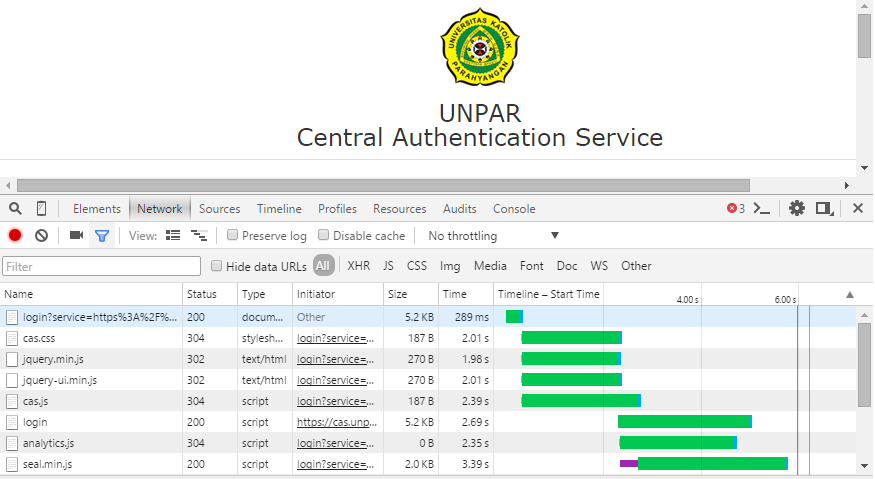
\includegraphics[scale=0.5]{Gambar/chrome-devtools}
	\caption{Chrome DevTools} 
	\label{fig:2_chrome_devtools}
\end{figure}

Pada subbab-subbab berikut akan dijelaskan mengenai dua panel dari DevTools.

\subsection{Elements}
Panel Elements memungkinkan untuk memperlihatkan informasi yang terstruktur tentang halaman yang sedang dibuka. HTML akan ditampilkan dalam bentuk pohon \textit{Document Object Model} (DOM). DOM adalah sebuah struktur seperti pohon yang dibuat oleh browser untuk menemukan elemen HTML \footnote{\url{http://try.jquery.com/}, diakses 24 September 2015}. Tampilan pohon DOM memperlihatkan struktur DOM dari halaman yang sedang dibuka. Pohon DOM adalah pohon dari node-node yang mewakili setiap elemen HTML seperti \texttt{<body>} dan \texttt{<p>}. 

Pemeriksaan elemen akan memperlihatkan node DOM dan CSS dari elemen yang dipilih pada \textit{browser}. Pemeriksaan elemen dapat dilakukan dengan cara klik kanan pada elemen yang ingin diperiksa kemudian pilih ``Inspect element''. Dengan melakukan pemeriksaan elemen, jendela panel Elements akan muncul. Sebagai contoh pada gambar \ref{fig:2_elements_panel}, saat melakukan ``Inspect element'' pada nama mahasiswa, panel Elements akan muncul dan menunjukkan pohon DOM dari halaman tersebut. Selain itu panel Elements juga menunjukkan CSS selector dari elemen tersebut yaitu \texttt{p.student-name}.

\begin{figure}[H]
	\centering
	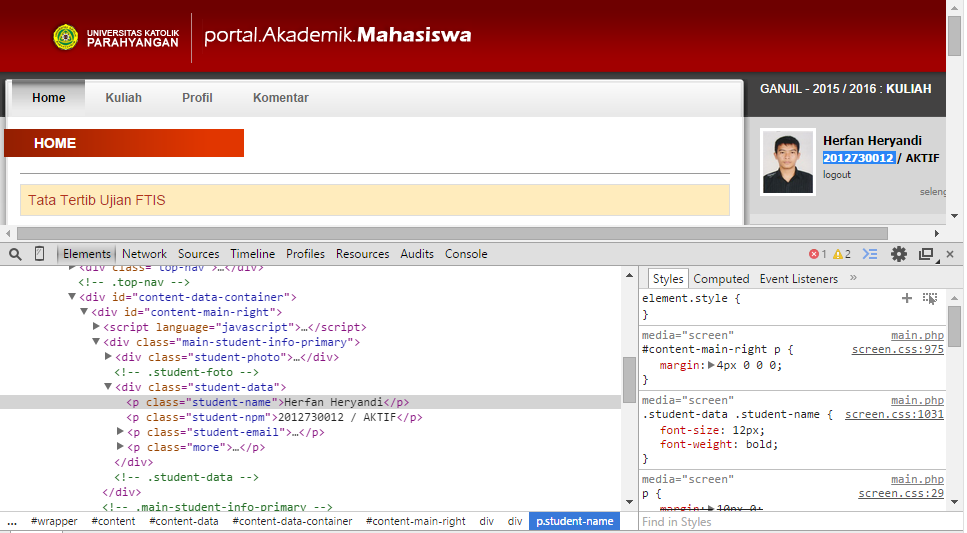
\includegraphics[scale=0.5]{Gambar/elements-panel}
	\caption{Panel Elements} 
	\label{fig:2_elements_panel}
\end{figure}

\subsection{Network}
Panel Network secara otomatis merekam semua aktivitas jaringan saat DevTools terbuka. Pertama kali dibuka, panel Network masih kosong. Halaman web harus dimuat ulang untuk mulai merekam aktivitas jaringan atau menunggu adanya aktivitas jaringan pada halaman web. Panel Network akan mencatat sumber daya dari aktivitas jaringan yang terekam. Setiap sumber daya akan ditambahkan ke dalam sebuah baris dalam tabel Network seperti pada gambar \ref{fig:2_network_panel} dengan rincian kolom sebagai berikut:
\begin{itemize}
	\item \textbf{Name dan Path}, nama dan URL dari sumber daya.
	\item \textbf{Method}, metode permintaan HTTP.
	\item \textbf{Status dan Text}, kode status HTTP dan pesan.
	\item \textbf{Domain}, domain dari sumber daya.
	\item \textbf{Type}, tipe sumber daya yang diminta.
	\item \textbf{Cookies}, banyaknya \textit{cookie} yang dikirim dalam permintaan.
	\item \textbf{Size dan Content}, \textit{size} merupakan ukuran dari \textit{header} dan \textit{body} jawaban yang dikirim server sedangkan \textit{content} merupakan ukuran konten sumber daya.
	\item \textbf{Timeline}, alur waktu dari seluruh aktivitas jaringan yang diminta.
\end{itemize}

\begin{figure}[H]
	\centering
	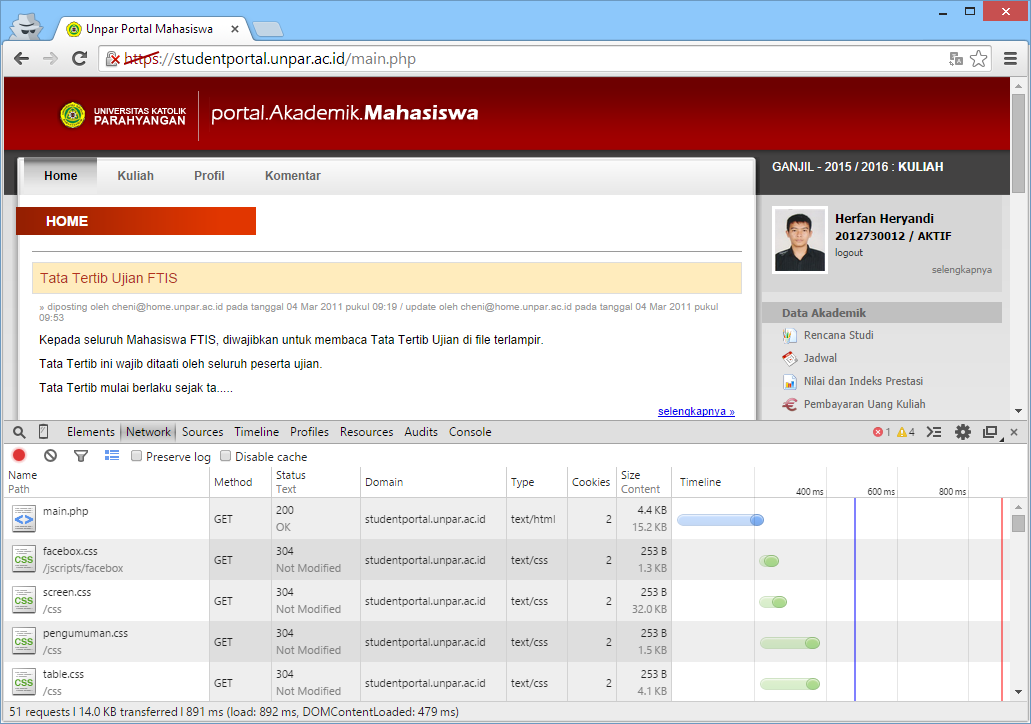
\includegraphics[scale=0.5]{Gambar/network-panel}
	\caption{Panel Network} 
	\label{fig:2_network_panel}
\end{figure}


Ketika nama sumber daya dalam tabel Network diklik, maka akan muncul tautan baru yang berisi rincian tambahan sebagai berikut:
\begin{itemize}
	\item \textbf{Header}\\
	Tautan Header menampilkan \textit{request} URL, \textit{request method}, \textit{status code}, HTTP \textit{response} dan \textit{request header} beserta nilainya, dan \textit{query string parameter}. HTTP header dapat ditampilkan secara terformat atau dalam bentuk sumber dengan mengklik tombol \textit{toggle} ``view parsed''/``view source''. Nilai-nilai parameter dapat ditampilkan dalam bentuk yang sudah didekodekan atau dalam bentuk URL yang dienkode dengan mengklik tombol \textit{toggle} ``view decoded''/``view URL encoded''. Sebagai contoh pada gambar \ref{fig:2_network_get} menampilkan \textit{header} pada metode permintaan GET sedangkan gambar \ref{fig:2_network_post} menampilkan \textit{header} pada metode permintaan POST.
	
\begin{figure}[H]
	\centering
	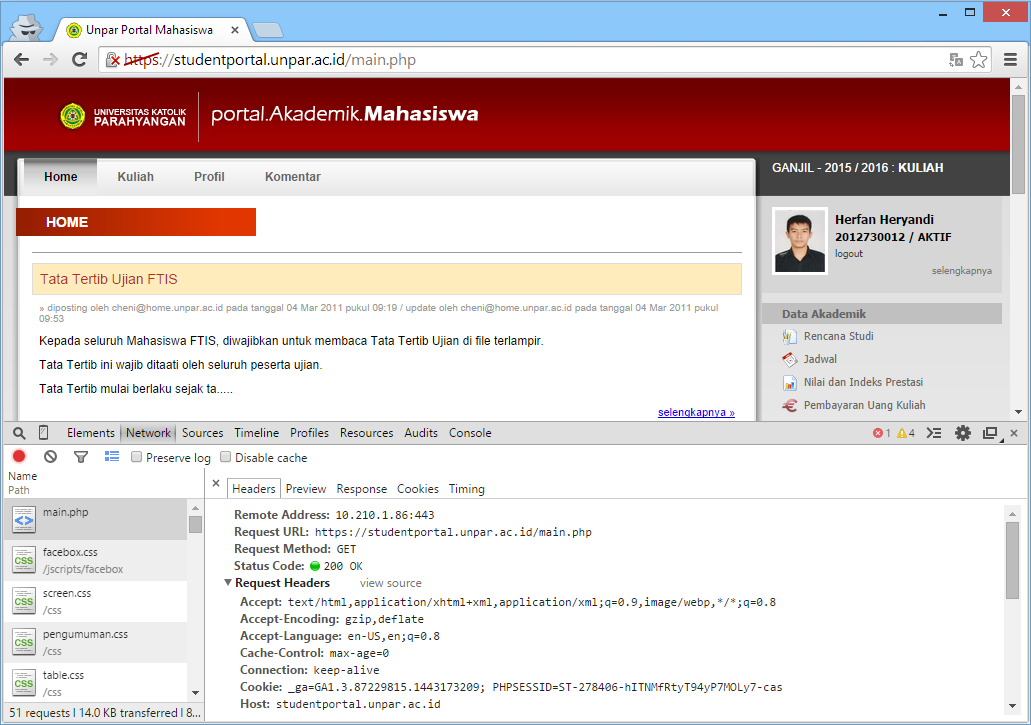
\includegraphics[scale=0.5]{Gambar/network-header}
	\caption{Contoh Tautan Header pada Metode Permintaan GET} 
	\label{fig:2_network_get}
\end{figure}

\begin{figure}[H]
	\centering
	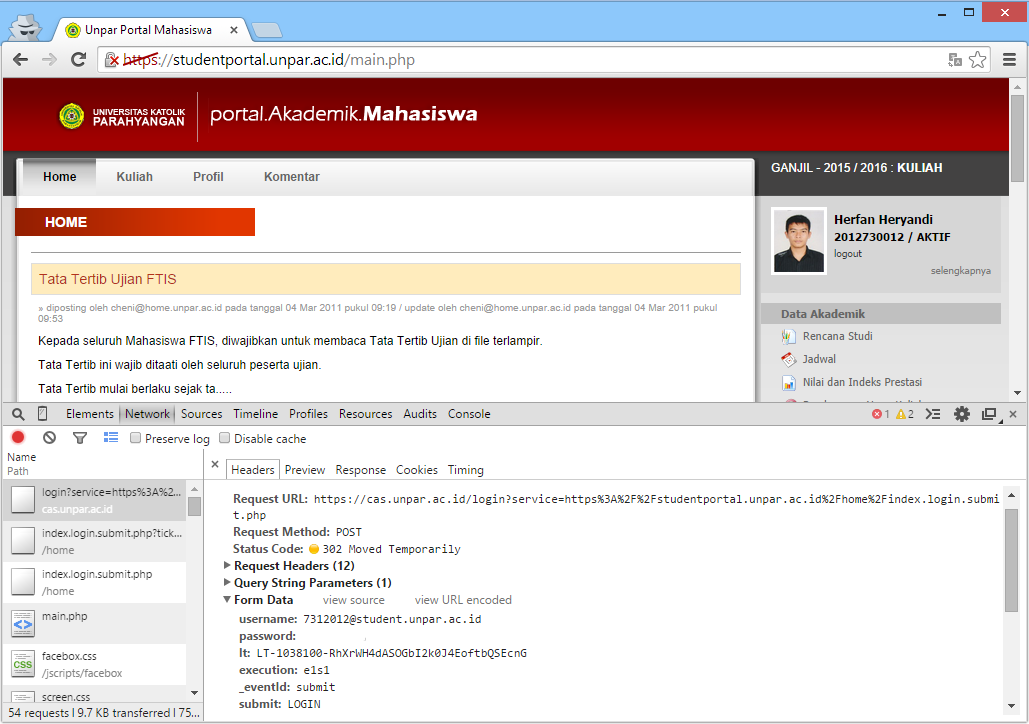
\includegraphics[scale=0.5]{Gambar/network-post}
	\caption{Contoh Tautan Header pada Metode Permintaan POST} 
	\label{fig:2_network_post}
\end{figure}

	\item \textbf{Preview}\\
	Tautan Preview menampilkan \textit{preview} sumber daya jika tersedia. Gambar \ref{fig:2_network_prev_available} menampilkan \textit{preview} yang tersedia pada sumber daya. Jika \textit{preview} tidak tersedia maka akan tampilan akan sama dengan jawaban seperti yang terlihat pada gambar \ref{fig:2_network_prev_notavailable}.
	
\begin{figure}[H]
	\centering
	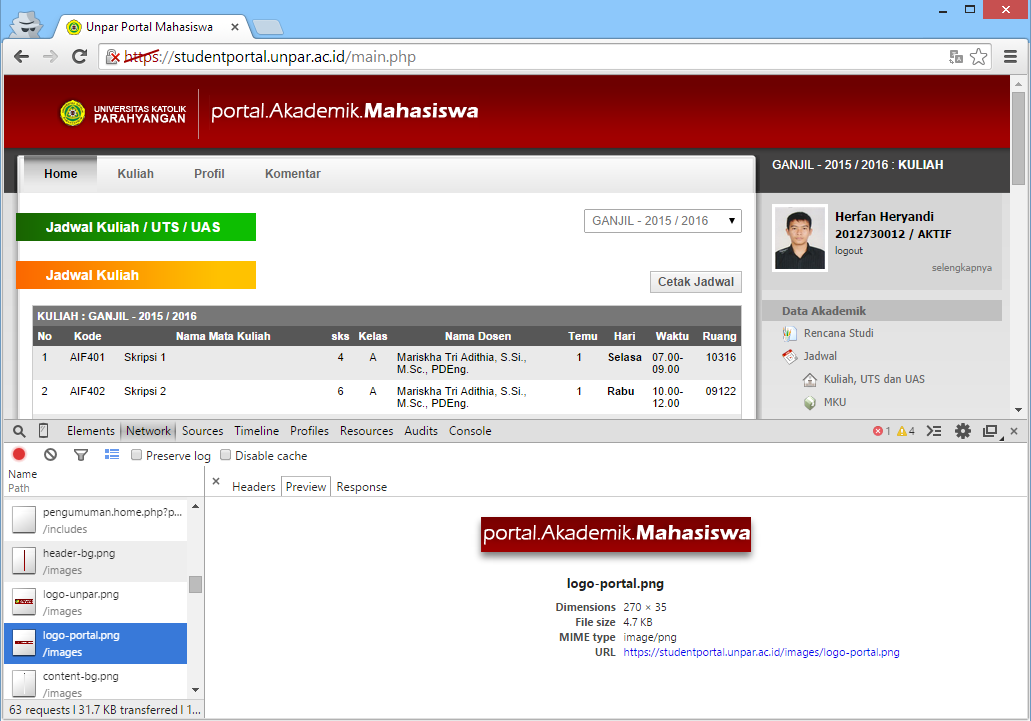
\includegraphics[scale=0.5]{Gambar/network-preview-available}
	\caption{Contoh \textit{Preview} yang Tersedia} 
	\label{fig:2_network_prev_available}
\end{figure}

\begin{figure}[H]
	\centering
	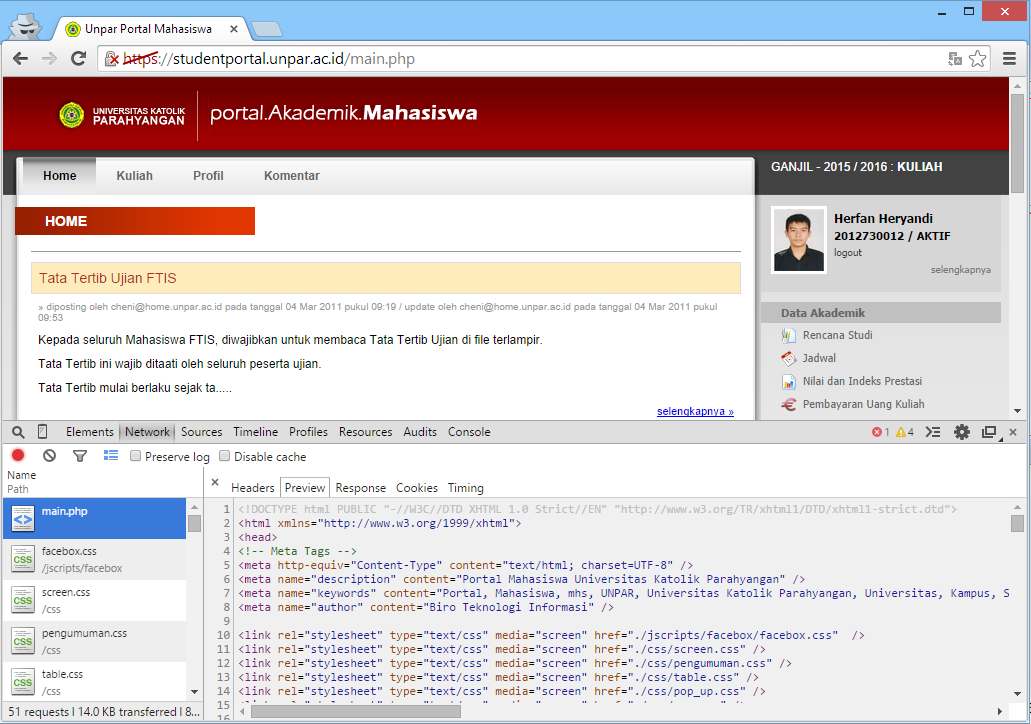
\includegraphics[scale=0.5]{Gambar/network-preview-notAvailable}
	\caption{Contoh \textit{Preview} yang Tidak Tersedia} 
	\label{fig:2_network_prev_notavailable}
\end{figure}

	\item \textbf{Response}\\
	Tautan Response berisi konten symber daya yang tidak terformat. Sebagai contoh pada gambar \ref{fig:2_network_response} menampilkan Tautan Response dari sumber daya \texttt{main.php}.
\begin{figure}[H]
	\centering
	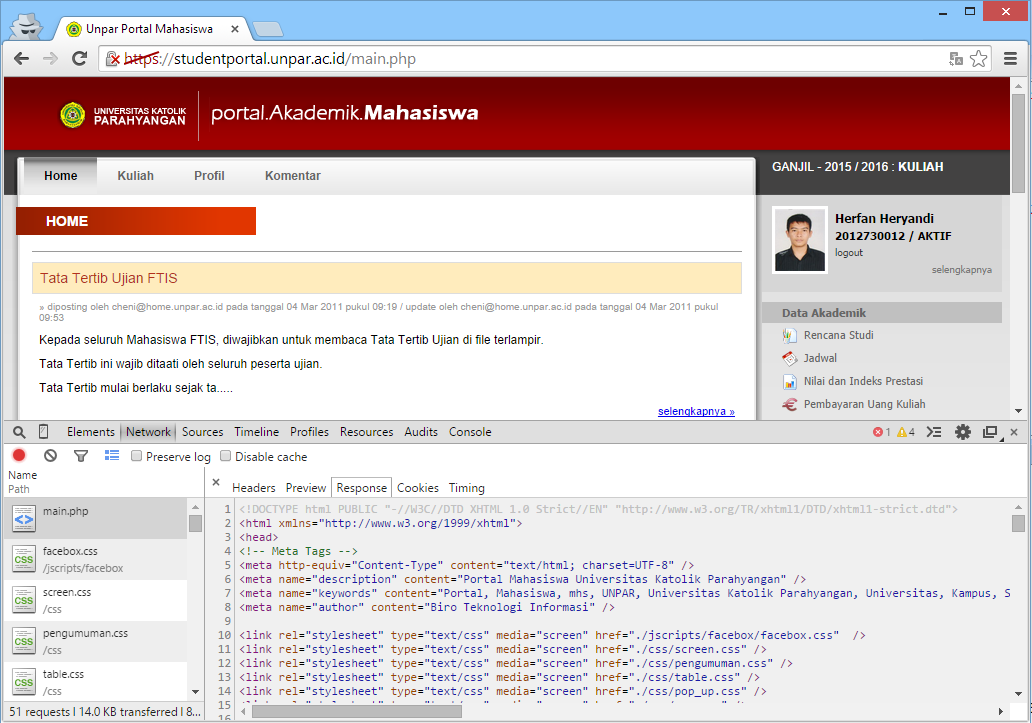
\includegraphics[scale=0.5]{Gambar/network-response}
	\caption{Contoh Tautan Response} 
	\label{fig:2_network_response}
\end{figure}

	\item \textbf{Cookies}\\
	Tautan Cookies menampilkan sebuah tabel yang terdiri dari seluruh \textit{cookie} yang ditransmisikan dalam \textit{header} permintaan dan jawaban HTTP. Contoh dari tabel \textit{cookie} dapat dilihat pada gambar \ref{fig:2_network_cookies} dengan rincian kolom sebagai berikut:
	\begin{itemize}
		\item \textbf{Name}, nama \textit{cookie}
		\item \textbf{Value}, nilai \textit{cookie}
		\item \textbf{Domain}, domain yang memiliki \textit{cookie}
		\item \textbf{Path}, URL asal \textit{cookie}
		\item \textbf{Expires/Max-Age}, batas akhir nilai \textit{cookie}
		\item \textbf{Size}, ukuran \textit{cookie} dalam byte
		\item \textbf{HTTP}, menunjukkan bahwa \textit{cookie} harus ditetapkan oleh browser dalam permintaan HTTP, dan tidak dapat diakses dengan JavaScript
		\item \textbf{Secure}, menunjukkan bahwa \textit{cookie} harus dikirim melalui koneksi yang aman
	\end{itemize}
	
\begin{figure}[H]
	\centering
	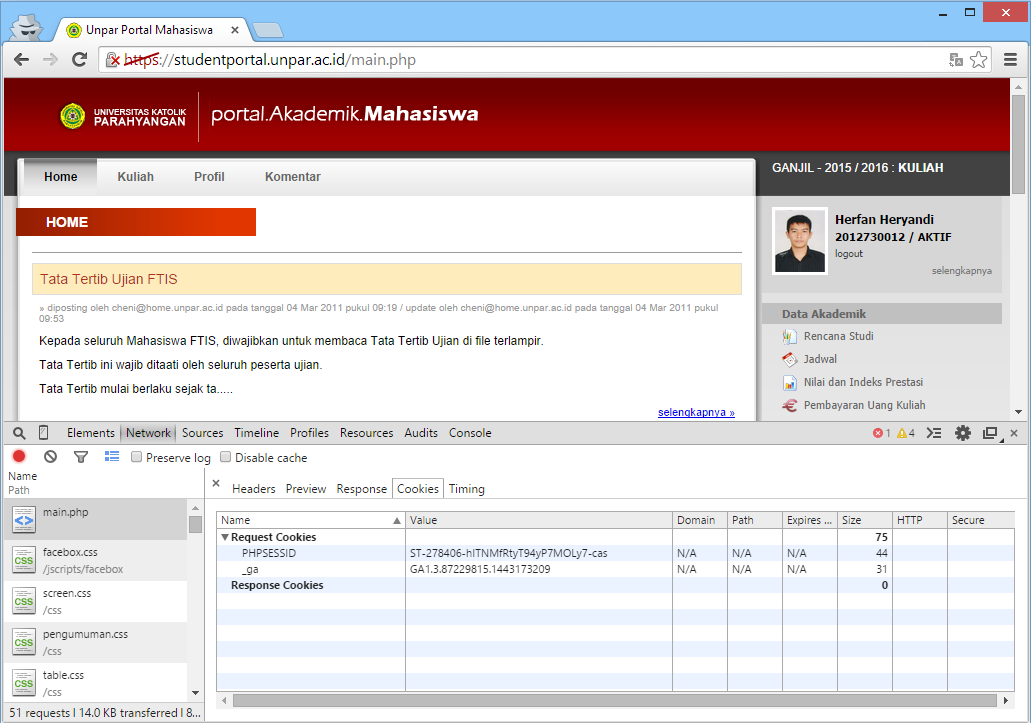
\includegraphics[scale=0.5]{Gambar/network-cookies}
	\caption{Contoh Tabel pada Tautan Cookie} 
	\label{fig:2_network_cookies}
\end{figure}

\end{itemize}

\section{Play Framework}
\label{sec:play}

Play Framework\cite{Leroux:2014} merupakan sebuah web \textit{framework} berbasis bahasa Java dan Scala. Play Framework juga menggunakan \textit{design pattern} Model-View-Controller (MVC) di mana \textit{model} dan \textit{controller} menggunakan bahasa Java sedangkan \textit{view} menggunakan bahasa Scala dan HTML. Struktur aplikasi Play Framework dapat dilihat pada gambar \ref{fig:2_play_dir}.
\begin{figure}[H]
	\centering
	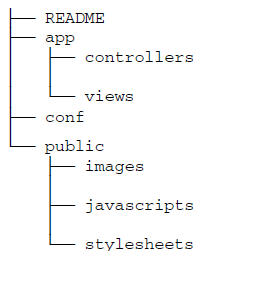
\includegraphics[scale=0.5]{Gambar/play-dir}
	\caption{Struktur Aplikasi Play Framework} 
	\label{fig:2_play_dir}
\end{figure}

Dalam direktori \texttt{conf}, terdapat file \texttt{routes}. Melalui \texttt{routes}, rute aplikasi dapat ditentukan dengan memetakan URL ke kode aplikasi. Setiap \texttt{route} memiliki tiga bagian yaitu HTTP \textit{method}, URL \textit{path}, dan \textit{action method}.  HTTP \textit{method} merupakan metode pengiriman HTTP. URL \textit{path} merupakan URL untuk mengakses halaman. \textit{Action method} merupakan \textit{method} yang menangani permintaan metode pengiriman HTTP. Sebagai contoh pada gambar \ref{fig:2_routes_example}, setiap permintaan GET pada URL \texttt{/list} akan ditangani oleh \textit{method} \texttt{list}() milik kelas \texttt{Products} yang terdapat pada \textit{package} \texttt{controllers}.

\begin{figure}[H]
	\centering
	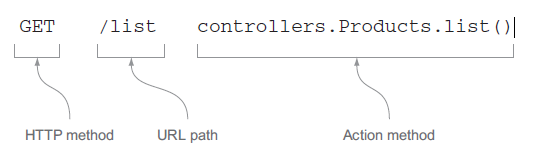
\includegraphics[scale=0.5]{Gambar/contoh-routes}
	\caption{Contoh Komponen \texttt{Route}\cite{Leroux:2014}} 
	\label{fig:2_routes_example}
\end{figure}

Direktori \texttt{app} merupakan sumber dari kode program seperti file Java dan \textit{view}. Saat pertama kali proyek Play Framework dibuat, direktori \texttt{app} berisi file-file seperti pada gambar \ref{fig:2_app_dir}. Dalam folder \texttt{controllers}, terdapat file \texttt{Application.java} yang berisi kode Java untuk menghasilkan halaman web. Kelas yang menangani permintaan HTTP dan mengembalikan hasil HTTP disebut kelas \textit{controller}. Dalam folder views terdapat dua file yaitu \texttt{index.scala.html} dan \texttt{main.scala.html} yang berfungsi untuk mendefinisikan halaman HTML. Setiap konten yang dihasilkan pada server dan dikirim ke klien dalam \textit{body} HTTP, seperti halaman HTML, disebut \textit{view}. Folder-folder yang terdapat dalam direktori \texttt{app} akan menjadi \textit{package} dalam kode Java.
\begin{figure}[H]
	\centering
	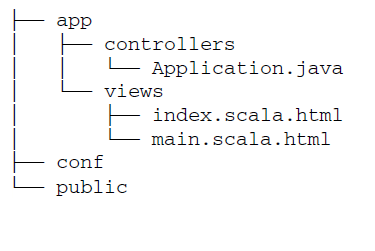
\includegraphics[scale=0.5]{Gambar/app-dir}
	\caption{Direktori \texttt{app} yang Dibangkitkan Play Framework\cite{Leroux:2014}} 
	\label{fig:2_app_dir}
\end{figure}


Direktori \texttt{public} berisi sumber yang dapat diakses secara langsung sebagai aset publik. Biasanya aset publik mendukung file selain aplikasi yang dibuat seperti gambar, \textit{stylesheet}, Javascript, dan halaman HTML statis. Aset publik tidak dihasilkan oleh aplikasi melainkan diatur secara langsung oleh pembuat program.

